\documentclass[12pt]{article}
\usepackage{amssymb}
\usepackage{amsmath}
\usepackage{amsthm}
\usepackage{mathtools}
\usepackage{array}
\usepackage{multirow}
\usepackage{colortbl}
\usepackage[dvipsnames]{xcolor}
\usepackage{graphicx}
  \DeclareGraphicsRule{*}{mps}{*}{}
%\usepackage{bbm}
\usepackage{marvosym}
\usepackage{enumerate}
\usepackage{txfonts}
\usepackage{paralist}
\usepackage{pdfpages}
\usepackage{multicol}
\usepackage{tikz}
\usepackage{siunitx}
\usepackage[normalem]{ulem}
\everymath{\displaystyle}

\usepackage[margin=.7in]{geometry}
%\usepackage{fullpage}

\setdefaultleftmargin{0pt}{}{}{}{}{}

\newcommand{\mblank}{\rule[-1ex]{8ex}{0.4pt}}
\definecolor{lightgray}{gray}{0.7}

\newenvironment{solution}
{\color{BrickRed}\textbf{Solution.} 
}
{\ignorespacesafterend}


\renewcommand{\thefootnote}{\fnsymbol{footnote}}

\hyphenpenalty=5000
\tolerance=1000
\setlength{\parindent}{0pt}

\begin{document}
\pagestyle{empty}
\begin{center}
\section*{MATH 210 -- Chapter 4 quiz}
\end{center}

\begin{enumerate}

\item (\textbf{P1}) 
Prove this theorem: For all natural numbers $n$, if $n^2$ is a multiple of 3, then $n$ is a multiple of 3.

\item (\textbf{P1 or P2?})
Prove or disprove: Every cycle is 2-colorable.

\item \textbf{(P3)} Construct a well-explained combinatorial proof of the following theorem:

For all natural numbers n, i, j, and k where $i+j+k=n$, $\frac{n!}{i! \cdot j! \cdot k!} = \binom{n}{i} \cdot \binom{n-i}{j}$.

Hint: You might think about words of a certain length made up of a certain number of certain letters.

\item \textbf{(P5)} Consider the following theorem: If $ab$ is even, then either $a$ is even or $b$ is even.

The following is an \textbf{incorrect} proof of the theorem:
\begin{quotation}
Assume that $a$ or $b$ is even. Without loss of generality, say that it's $a$. Then, by definition, we can write $a = 2k$ for some $k\in\mathbb{N}$. Thus:
\begin{align*}
    ab &= (2k) b \\
    &= 2kb \\
    &= 2(kb) = 2j,
\end{align*}
where $j = kb$ is a natural number. Therefore, by definition, $ab$ is even. \qed
\end{quotation}
Carefully explain what is wrong with this proof attempt.

Optional, for \textbf{P1} credit: Provide a \textbf{correct} proof of this theorem.


\item (\textbf{S1})
Here are two sets, $A$ and $B$, written in set-builder notation.  
\begin{center}
$A=\{x: \exists n \in \mathbb{Z}, x=3n+1\}$ \\
$B=\{x: \exists n \in \mathbb{Z}, x=3n-2\}$
\end{center}

Which of the following, if any, are true: $A \subset B, B \subset A, A=B$. Explain your answer.


\item \textbf{(S2)} Draw a Venn diagram to represent each of the following:
\begin{enumerate}
    \item $A\cup \overline{B}$
    \item $A\cap\overline{B}$
    \item $A\cap(B\cup C)$
    \item $(A \cap B) \cup C$
    \item $\overline{A} \cap B \cap \overline{C}$
\end{enumerate}

\item Let $A = \{1,2,3,4\}$ and $B = \{x,y,z,w\}$. 
\begin{enumerate}
    \item \textbf{(S3)} Give an example of a function $f:A\to B$ that is not surjective. 
    
    \item \textbf{(P1 or P2?)} Prove or disprove: a function $f:A\to B$ is injective if and only if it is surjective.
    
\end{enumerate}

\item\textbf{(S4, S5)} Consider a relation R on the set of all members of a basketball team defined as follows:
\begin{center}
  $aRb$  if and only if $a$ and $b$ are the same height  
\end{center}
\begin{enumerate}
    \item Is relation R an equivalence relation? Explain.
    \item What does each equivalence class look like?
\end{enumerate}

\item
\textbf{(L1, L3)} Consider the following statement about the relationship between two sets, A and B, of natural numbers:


        \[\exists x \in \mathbb{N},\ x \in A \land x \not\in B \]
\begin{enumerate}
    \item 
    Write the formal simplified negation of this statement.
    
    \item
    Explain the meaning of the original statement and the meaning of its negation using familiar set relations.
    
\end{enumerate}

\item \textbf{(L1, L3)} Consider the statement: ``If a graph is planar, then $v-e+f=2$.''
\begin{enumerate}
    \item Write the converse of the statement.
    \item Write the contrapositive of the statement.
    \item Write the negation of the statement.
    \item Is the original statement true? Is the converse true? Is the contrapositive true? Is the negation true? Explain.
\end{enumerate}

\item
\textbf{(L2)} Are the two compound logical statements below logically equivalent or not? Include a truth table and a clear explanation.
\[
(P \land Q) \rightarrow R \hspace{40pt} \lnot P \lor \lnot Q \lor R
\]

\item (\textbf{C1}) Consider binary strings of length ten.

\begin{enumerate}
    \item How many strings are there total?
    \item How many strings have exactly four 1's?
    \item How many strings have an even number of 1's?
    \item How many strings begin with a 1 or end with a 1?
\end{enumerate}

\item \textbf{(C1, C2, C3)} For each of the following counting problems, say whether the answer is $\binom{10}{4}$ or $P(10,4)$ or neither and explain why. If you answer is “neither,” say what the answer should be instead.

\begin{enumerate}
    \item Out of a group of 10 classmates, how many ways can you rank your top 4 friends?
    
    \item How many ways are there to distribute 10 apples among 4 children?
    
    \item How many surjective functions are there from $\{1,2,3,...,10\}$ to $\{a,b,c,d\}$?
    
\end{enumerate}

\item \textbf{(Q1)} In the song The Twelve Days of Christmas, my true love gave to me first 1 gift, then 2 gifts and 1 gift, then 3 gifts, 2 gifts and 1 gift, and so on until the twelfth day. 
\begin{enumerate}
    \item Use the reverse-and-add technique to find a closed formula for $a_n$, the number of gifts I received on the $n$th day.
    \item How many gifts did my true love give me all together during the twelve days? \\(Hint: use the result of part (a)).
\end{enumerate}

\item (\textbf{Q1, P4}) Consider the sequence of partial sums of \textbf{squares} of Fibonacci numbers: 
\[F_1^2,\ F_1^2 + F_2^2,\ F_1^2+F_2^2 + F_3^2,\ \ldots\ , F_1^2+F_2^2 + \ldots + F_n^2,\ \ldots\]
Just to check that we're all on the same page, this sequence starts 1, 2, 6, 15, 40, \ldots
\begin{enumerate}
    \item Guess a formula for the $n$th partial sum, in terms of Fibonacci numbers. \\(\textbf{Hint}: Write each term as a product.) 
    
    \item Prove your formula is correct by mathematical induction.
    
    \item Explain what this problem has to do with the following picture.
\begin{center}
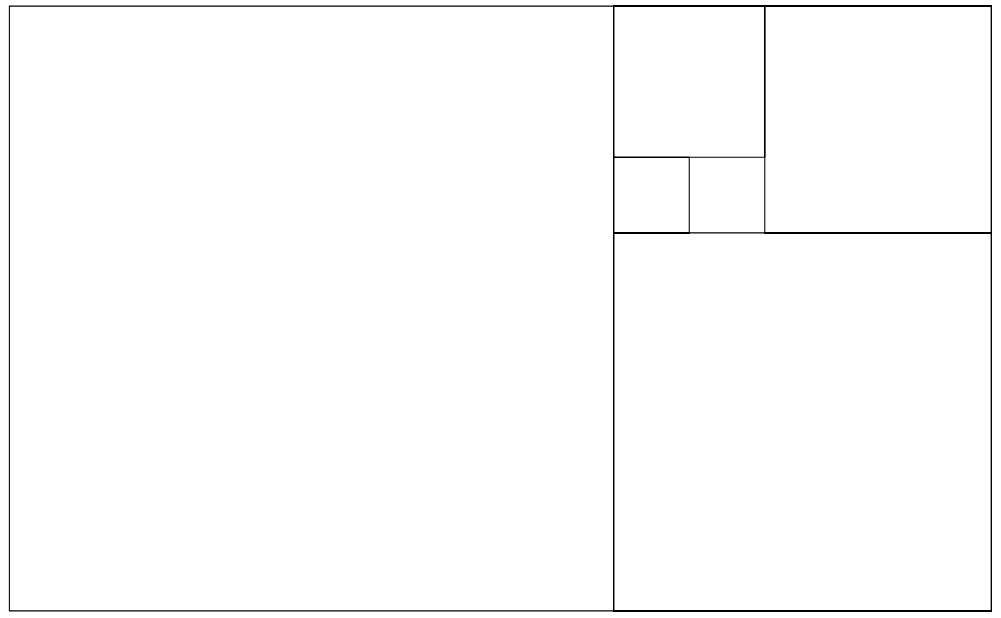
\includegraphics[width=0.5\textwidth]{golden-rectangles.png}
\end{center}
    
\end{enumerate}


\item \textbf{(Q1, Q2)}  Your magic chocolate bunnies reproduce like rabbits: every large bunny produces 2 new mini bunnies each day, and each day every mini bunny born the previous day grows into a large bunny. Assume you start with 2 mini bunnies and no bunny ever dies (or gets eaten).
\begin{enumerate}
    \item Say that $a_n$ is the total number of bunnies (both mini and large) you have on the $n$th day. Write out the first few terms of this sequence.
    \item Give a recursive definition of the sequence and explain why it is correct. 
    \item Find a closed formula for the $n$th term of the sequence.
\end{enumerate}

\item \textbf{(Q2)} Consider the recurrence relation $a_n = 4a_{n-1} - 4a_{n-2}$.
\begin{enumerate}
    \item Find the general solution to the recurrence relation (beware the repeated root).
    
    \item Find the solution when $a_0 = 1$ and $a_1 = 2$.
    
\end{enumerate}

\item Consider the graph $G = (V, E)$ with vertex set $V = \{a,b,c,d,e,f,g\}$ and edge set $E = \{ab, ac, af, bg, cd, ce\}$ (here we're using some shorthand notation where, for instance, $ab$ is an edge between $a$ and $b$).

\begin{enumerate}
    \item \textbf{(G1)} Draw a representation of $G$.
    \item \textbf{(G2)} Is $G$ isomorphic to the graph $H = (W, F)$ with vertex set $W = \{t, u, v, w, x, y, z\}$ and edge set $F = \{tz, uv, uy, uz, vw, vx\}$? If yes, give the isomorphism; if not, explain how you know.
    \item \textbf{(G3)} What kind of graph is $G$? Is it complete? Is it a tree? Bipartite? Planar? Explain how you know.
    \item \textbf{(G3)} Does $G$ have an Euler path? How about an Euler circuit? Explain how you know.
    \item \textbf{(G4)} What is the chromatic number of $G$?
\end{enumerate}

\item Consider the graph below.

\begin{tikzpicture}
  [scale=.8,auto=left,every node/.style={circle,draw}]
  \node (n6) at (1,10) {6};
  \node (n4) at (4,8)  {4};
  \node (n5) at (8,9)  {5};
  \node (n1) at (11,8) {1};
  \node (n2) at (9,6)  {2};
  \node (n3) at (5,5)  {3};

  \foreach \from/\to in {n6/n4,n4/n5,n5/n1,n1/n2,n2/n5,n2/n3,n3/n4}
    \draw (\from) -- (\to);

\end{tikzpicture}

\begin{enumerate}
    \item \textbf{(G1)} Write down the vertex set and the edge set.
    
    \item \textbf{(G3)} Is the graph a tree, complete, bipartite, planar, or have an Euler circuit? Explain. 
    
    \item \textbf{(G4)} What is the chromatic number of this graph? Illustrate by providing a smallest proper coloring.
    
\end{enumerate}

\item \textbf{(G2)} Below are two graphs, $G$ and $G'$, with vertices and edges labeled. Are these graphs isomorphic? Explain your answer.

\begin{center}
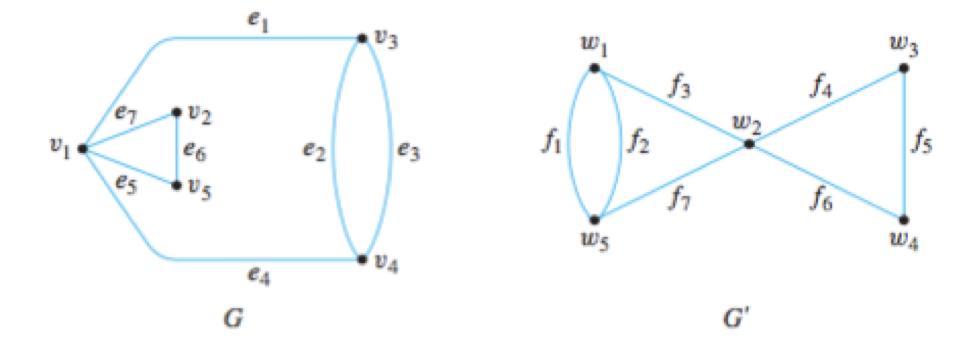
\includegraphics[width=0.7\textwidth]{graphs_picture.png}
\end{center}

\end{enumerate}
\end{document}